
% Default to the notebook output style

    


% Inherit from the specified cell style.




    
\documentclass[11pt]{article}

    
    
    \usepackage[T1]{fontenc}
    % Nicer default font (+ math font) than Computer Modern for most use cases
    \usepackage{mathpazo}

    % Basic figure setup, for now with no caption control since it's done
    % automatically by Pandoc (which extracts ![](path) syntax from Markdown).
    \usepackage{graphicx}
    % We will generate all images so they have a width \maxwidth. This means
    % that they will get their normal width if they fit onto the page, but
    % are scaled down if they would overflow the margins.
    \makeatletter
    \def\maxwidth{\ifdim\Gin@nat@width>\linewidth\linewidth
    \else\Gin@nat@width\fi}
    \makeatother
    \let\Oldincludegraphics\includegraphics
    % Set max figure width to be 80% of text width, for now hardcoded.
    \renewcommand{\includegraphics}[1]{\Oldincludegraphics[width=.8\maxwidth]{#1}}
    % Ensure that by default, figures have no caption (until we provide a
    % proper Figure object with a Caption API and a way to capture that
    % in the conversion process - todo).
    \usepackage{caption}
    \DeclareCaptionLabelFormat{nolabel}{}
    \captionsetup{labelformat=nolabel}

    \usepackage{adjustbox} % Used to constrain images to a maximum size 
    \usepackage{xcolor} % Allow colors to be defined
    \usepackage{enumerate} % Needed for markdown enumerations to work
    \usepackage{geometry} % Used to adjust the document margins
    \usepackage{amsmath} % Equations
    \usepackage{amssymb} % Equations
    \usepackage{textcomp} % defines textquotesingle
    % Hack from http://tex.stackexchange.com/a/47451/13684:
    \AtBeginDocument{%
        \def\PYZsq{\textquotesingle}% Upright quotes in Pygmentized code
    }
    \usepackage{upquote} % Upright quotes for verbatim code
    \usepackage{eurosym} % defines \euro
    \usepackage[mathletters]{ucs} % Extended unicode (utf-8) support
    \usepackage[utf8x]{inputenc} % Allow utf-8 characters in the tex document
    \usepackage{fancyvrb} % verbatim replacement that allows latex
    \usepackage{grffile} % extends the file name processing of package graphics 
                         % to support a larger range 
    % The hyperref package gives us a pdf with properly built
    % internal navigation ('pdf bookmarks' for the table of contents,
    % internal cross-reference links, web links for URLs, etc.)
    \usepackage{hyperref}
    \usepackage{longtable} % longtable support required by pandoc >1.10
    \usepackage{booktabs}  % table support for pandoc > 1.12.2
    \usepackage[inline]{enumitem} % IRkernel/repr support (it uses the enumerate* environment)
    \usepackage[normalem]{ulem} % ulem is needed to support strikethroughs (\sout)
                                % normalem makes italics be italics, not underlines
    

    
    
    % Colors for the hyperref package
    \definecolor{urlcolor}{rgb}{0,.145,.698}
    \definecolor{linkcolor}{rgb}{.71,0.21,0.01}
    \definecolor{citecolor}{rgb}{.12,.54,.11}

    % ANSI colors
    \definecolor{ansi-black}{HTML}{3E424D}
    \definecolor{ansi-black-intense}{HTML}{282C36}
    \definecolor{ansi-red}{HTML}{E75C58}
    \definecolor{ansi-red-intense}{HTML}{B22B31}
    \definecolor{ansi-green}{HTML}{00A250}
    \definecolor{ansi-green-intense}{HTML}{007427}
    \definecolor{ansi-yellow}{HTML}{DDB62B}
    \definecolor{ansi-yellow-intense}{HTML}{B27D12}
    \definecolor{ansi-blue}{HTML}{208FFB}
    \definecolor{ansi-blue-intense}{HTML}{0065CA}
    \definecolor{ansi-magenta}{HTML}{D160C4}
    \definecolor{ansi-magenta-intense}{HTML}{A03196}
    \definecolor{ansi-cyan}{HTML}{60C6C8}
    \definecolor{ansi-cyan-intense}{HTML}{258F8F}
    \definecolor{ansi-white}{HTML}{C5C1B4}
    \definecolor{ansi-white-intense}{HTML}{A1A6B2}

    % commands and environments needed by pandoc snippets
    % extracted from the output of `pandoc -s`
    \providecommand{\tightlist}{%
      \setlength{\itemsep}{0pt}\setlength{\parskip}{0pt}}
    \DefineVerbatimEnvironment{Highlighting}{Verbatim}{commandchars=\\\{\}}
    % Add ',fontsize=\small' for more characters per line
    \newenvironment{Shaded}{}{}
    \newcommand{\KeywordTok}[1]{\textcolor[rgb]{0.00,0.44,0.13}{\textbf{{#1}}}}
    \newcommand{\DataTypeTok}[1]{\textcolor[rgb]{0.56,0.13,0.00}{{#1}}}
    \newcommand{\DecValTok}[1]{\textcolor[rgb]{0.25,0.63,0.44}{{#1}}}
    \newcommand{\BaseNTok}[1]{\textcolor[rgb]{0.25,0.63,0.44}{{#1}}}
    \newcommand{\FloatTok}[1]{\textcolor[rgb]{0.25,0.63,0.44}{{#1}}}
    \newcommand{\CharTok}[1]{\textcolor[rgb]{0.25,0.44,0.63}{{#1}}}
    \newcommand{\StringTok}[1]{\textcolor[rgb]{0.25,0.44,0.63}{{#1}}}
    \newcommand{\CommentTok}[1]{\textcolor[rgb]{0.38,0.63,0.69}{\textit{{#1}}}}
    \newcommand{\OtherTok}[1]{\textcolor[rgb]{0.00,0.44,0.13}{{#1}}}
    \newcommand{\AlertTok}[1]{\textcolor[rgb]{1.00,0.00,0.00}{\textbf{{#1}}}}
    \newcommand{\FunctionTok}[1]{\textcolor[rgb]{0.02,0.16,0.49}{{#1}}}
    \newcommand{\RegionMarkerTok}[1]{{#1}}
    \newcommand{\ErrorTok}[1]{\textcolor[rgb]{1.00,0.00,0.00}{\textbf{{#1}}}}
    \newcommand{\NormalTok}[1]{{#1}}
    
    % Additional commands for more recent versions of Pandoc
    \newcommand{\ConstantTok}[1]{\textcolor[rgb]{0.53,0.00,0.00}{{#1}}}
    \newcommand{\SpecialCharTok}[1]{\textcolor[rgb]{0.25,0.44,0.63}{{#1}}}
    \newcommand{\VerbatimStringTok}[1]{\textcolor[rgb]{0.25,0.44,0.63}{{#1}}}
    \newcommand{\SpecialStringTok}[1]{\textcolor[rgb]{0.73,0.40,0.53}{{#1}}}
    \newcommand{\ImportTok}[1]{{#1}}
    \newcommand{\DocumentationTok}[1]{\textcolor[rgb]{0.73,0.13,0.13}{\textit{{#1}}}}
    \newcommand{\AnnotationTok}[1]{\textcolor[rgb]{0.38,0.63,0.69}{\textbf{\textit{{#1}}}}}
    \newcommand{\CommentVarTok}[1]{\textcolor[rgb]{0.38,0.63,0.69}{\textbf{\textit{{#1}}}}}
    \newcommand{\VariableTok}[1]{\textcolor[rgb]{0.10,0.09,0.49}{{#1}}}
    \newcommand{\ControlFlowTok}[1]{\textcolor[rgb]{0.00,0.44,0.13}{\textbf{{#1}}}}
    \newcommand{\OperatorTok}[1]{\textcolor[rgb]{0.40,0.40,0.40}{{#1}}}
    \newcommand{\BuiltInTok}[1]{{#1}}
    \newcommand{\ExtensionTok}[1]{{#1}}
    \newcommand{\PreprocessorTok}[1]{\textcolor[rgb]{0.74,0.48,0.00}{{#1}}}
    \newcommand{\AttributeTok}[1]{\textcolor[rgb]{0.49,0.56,0.16}{{#1}}}
    \newcommand{\InformationTok}[1]{\textcolor[rgb]{0.38,0.63,0.69}{\textbf{\textit{{#1}}}}}
    \newcommand{\WarningTok}[1]{\textcolor[rgb]{0.38,0.63,0.69}{\textbf{\textit{{#1}}}}}
    
    
    % Define a nice break command that doesn't care if a line doesn't already
    % exist.
    \def\br{\hspace*{\fill} \\* }
    % Math Jax compatability definitions
    \def\gt{>}
    \def\lt{<}
    % Document parameters
    \title{GGS560 Homework 10}
    
    
    

    % Pygments definitions
    
\makeatletter
\def\PY@reset{\let\PY@it=\relax \let\PY@bf=\relax%
    \let\PY@ul=\relax \let\PY@tc=\relax%
    \let\PY@bc=\relax \let\PY@ff=\relax}
\def\PY@tok#1{\csname PY@tok@#1\endcsname}
\def\PY@toks#1+{\ifx\relax#1\empty\else%
    \PY@tok{#1}\expandafter\PY@toks\fi}
\def\PY@do#1{\PY@bc{\PY@tc{\PY@ul{%
    \PY@it{\PY@bf{\PY@ff{#1}}}}}}}
\def\PY#1#2{\PY@reset\PY@toks#1+\relax+\PY@do{#2}}

\expandafter\def\csname PY@tok@sa\endcsname{\def\PY@tc##1{\textcolor[rgb]{0.73,0.13,0.13}{##1}}}
\expandafter\def\csname PY@tok@s2\endcsname{\def\PY@tc##1{\textcolor[rgb]{0.73,0.13,0.13}{##1}}}
\expandafter\def\csname PY@tok@w\endcsname{\def\PY@tc##1{\textcolor[rgb]{0.73,0.73,0.73}{##1}}}
\expandafter\def\csname PY@tok@sd\endcsname{\let\PY@it=\textit\def\PY@tc##1{\textcolor[rgb]{0.73,0.13,0.13}{##1}}}
\expandafter\def\csname PY@tok@nf\endcsname{\def\PY@tc##1{\textcolor[rgb]{0.00,0.00,1.00}{##1}}}
\expandafter\def\csname PY@tok@bp\endcsname{\def\PY@tc##1{\textcolor[rgb]{0.00,0.50,0.00}{##1}}}
\expandafter\def\csname PY@tok@kt\endcsname{\def\PY@tc##1{\textcolor[rgb]{0.69,0.00,0.25}{##1}}}
\expandafter\def\csname PY@tok@c\endcsname{\let\PY@it=\textit\def\PY@tc##1{\textcolor[rgb]{0.25,0.50,0.50}{##1}}}
\expandafter\def\csname PY@tok@nn\endcsname{\let\PY@bf=\textbf\def\PY@tc##1{\textcolor[rgb]{0.00,0.00,1.00}{##1}}}
\expandafter\def\csname PY@tok@gr\endcsname{\def\PY@tc##1{\textcolor[rgb]{1.00,0.00,0.00}{##1}}}
\expandafter\def\csname PY@tok@gi\endcsname{\def\PY@tc##1{\textcolor[rgb]{0.00,0.63,0.00}{##1}}}
\expandafter\def\csname PY@tok@si\endcsname{\let\PY@bf=\textbf\def\PY@tc##1{\textcolor[rgb]{0.73,0.40,0.53}{##1}}}
\expandafter\def\csname PY@tok@il\endcsname{\def\PY@tc##1{\textcolor[rgb]{0.40,0.40,0.40}{##1}}}
\expandafter\def\csname PY@tok@gu\endcsname{\let\PY@bf=\textbf\def\PY@tc##1{\textcolor[rgb]{0.50,0.00,0.50}{##1}}}
\expandafter\def\csname PY@tok@mo\endcsname{\def\PY@tc##1{\textcolor[rgb]{0.40,0.40,0.40}{##1}}}
\expandafter\def\csname PY@tok@mh\endcsname{\def\PY@tc##1{\textcolor[rgb]{0.40,0.40,0.40}{##1}}}
\expandafter\def\csname PY@tok@no\endcsname{\def\PY@tc##1{\textcolor[rgb]{0.53,0.00,0.00}{##1}}}
\expandafter\def\csname PY@tok@ni\endcsname{\let\PY@bf=\textbf\def\PY@tc##1{\textcolor[rgb]{0.60,0.60,0.60}{##1}}}
\expandafter\def\csname PY@tok@sh\endcsname{\def\PY@tc##1{\textcolor[rgb]{0.73,0.13,0.13}{##1}}}
\expandafter\def\csname PY@tok@gp\endcsname{\let\PY@bf=\textbf\def\PY@tc##1{\textcolor[rgb]{0.00,0.00,0.50}{##1}}}
\expandafter\def\csname PY@tok@ch\endcsname{\let\PY@it=\textit\def\PY@tc##1{\textcolor[rgb]{0.25,0.50,0.50}{##1}}}
\expandafter\def\csname PY@tok@nt\endcsname{\let\PY@bf=\textbf\def\PY@tc##1{\textcolor[rgb]{0.00,0.50,0.00}{##1}}}
\expandafter\def\csname PY@tok@cpf\endcsname{\let\PY@it=\textit\def\PY@tc##1{\textcolor[rgb]{0.25,0.50,0.50}{##1}}}
\expandafter\def\csname PY@tok@cm\endcsname{\let\PY@it=\textit\def\PY@tc##1{\textcolor[rgb]{0.25,0.50,0.50}{##1}}}
\expandafter\def\csname PY@tok@ow\endcsname{\let\PY@bf=\textbf\def\PY@tc##1{\textcolor[rgb]{0.67,0.13,1.00}{##1}}}
\expandafter\def\csname PY@tok@se\endcsname{\let\PY@bf=\textbf\def\PY@tc##1{\textcolor[rgb]{0.73,0.40,0.13}{##1}}}
\expandafter\def\csname PY@tok@cp\endcsname{\def\PY@tc##1{\textcolor[rgb]{0.74,0.48,0.00}{##1}}}
\expandafter\def\csname PY@tok@nl\endcsname{\def\PY@tc##1{\textcolor[rgb]{0.63,0.63,0.00}{##1}}}
\expandafter\def\csname PY@tok@nc\endcsname{\let\PY@bf=\textbf\def\PY@tc##1{\textcolor[rgb]{0.00,0.00,1.00}{##1}}}
\expandafter\def\csname PY@tok@dl\endcsname{\def\PY@tc##1{\textcolor[rgb]{0.73,0.13,0.13}{##1}}}
\expandafter\def\csname PY@tok@gt\endcsname{\def\PY@tc##1{\textcolor[rgb]{0.00,0.27,0.87}{##1}}}
\expandafter\def\csname PY@tok@kd\endcsname{\let\PY@bf=\textbf\def\PY@tc##1{\textcolor[rgb]{0.00,0.50,0.00}{##1}}}
\expandafter\def\csname PY@tok@vg\endcsname{\def\PY@tc##1{\textcolor[rgb]{0.10,0.09,0.49}{##1}}}
\expandafter\def\csname PY@tok@ss\endcsname{\def\PY@tc##1{\textcolor[rgb]{0.10,0.09,0.49}{##1}}}
\expandafter\def\csname PY@tok@err\endcsname{\def\PY@bc##1{\setlength{\fboxsep}{0pt}\fcolorbox[rgb]{1.00,0.00,0.00}{1,1,1}{\strut ##1}}}
\expandafter\def\csname PY@tok@go\endcsname{\def\PY@tc##1{\textcolor[rgb]{0.53,0.53,0.53}{##1}}}
\expandafter\def\csname PY@tok@vc\endcsname{\def\PY@tc##1{\textcolor[rgb]{0.10,0.09,0.49}{##1}}}
\expandafter\def\csname PY@tok@vm\endcsname{\def\PY@tc##1{\textcolor[rgb]{0.10,0.09,0.49}{##1}}}
\expandafter\def\csname PY@tok@nd\endcsname{\def\PY@tc##1{\textcolor[rgb]{0.67,0.13,1.00}{##1}}}
\expandafter\def\csname PY@tok@kn\endcsname{\let\PY@bf=\textbf\def\PY@tc##1{\textcolor[rgb]{0.00,0.50,0.00}{##1}}}
\expandafter\def\csname PY@tok@sr\endcsname{\def\PY@tc##1{\textcolor[rgb]{0.73,0.40,0.53}{##1}}}
\expandafter\def\csname PY@tok@mb\endcsname{\def\PY@tc##1{\textcolor[rgb]{0.40,0.40,0.40}{##1}}}
\expandafter\def\csname PY@tok@gd\endcsname{\def\PY@tc##1{\textcolor[rgb]{0.63,0.00,0.00}{##1}}}
\expandafter\def\csname PY@tok@vi\endcsname{\def\PY@tc##1{\textcolor[rgb]{0.10,0.09,0.49}{##1}}}
\expandafter\def\csname PY@tok@sx\endcsname{\def\PY@tc##1{\textcolor[rgb]{0.00,0.50,0.00}{##1}}}
\expandafter\def\csname PY@tok@s1\endcsname{\def\PY@tc##1{\textcolor[rgb]{0.73,0.13,0.13}{##1}}}
\expandafter\def\csname PY@tok@gs\endcsname{\let\PY@bf=\textbf}
\expandafter\def\csname PY@tok@nv\endcsname{\def\PY@tc##1{\textcolor[rgb]{0.10,0.09,0.49}{##1}}}
\expandafter\def\csname PY@tok@kp\endcsname{\def\PY@tc##1{\textcolor[rgb]{0.00,0.50,0.00}{##1}}}
\expandafter\def\csname PY@tok@o\endcsname{\def\PY@tc##1{\textcolor[rgb]{0.40,0.40,0.40}{##1}}}
\expandafter\def\csname PY@tok@s\endcsname{\def\PY@tc##1{\textcolor[rgb]{0.73,0.13,0.13}{##1}}}
\expandafter\def\csname PY@tok@nb\endcsname{\def\PY@tc##1{\textcolor[rgb]{0.00,0.50,0.00}{##1}}}
\expandafter\def\csname PY@tok@sc\endcsname{\def\PY@tc##1{\textcolor[rgb]{0.73,0.13,0.13}{##1}}}
\expandafter\def\csname PY@tok@na\endcsname{\def\PY@tc##1{\textcolor[rgb]{0.49,0.56,0.16}{##1}}}
\expandafter\def\csname PY@tok@cs\endcsname{\let\PY@it=\textit\def\PY@tc##1{\textcolor[rgb]{0.25,0.50,0.50}{##1}}}
\expandafter\def\csname PY@tok@c1\endcsname{\let\PY@it=\textit\def\PY@tc##1{\textcolor[rgb]{0.25,0.50,0.50}{##1}}}
\expandafter\def\csname PY@tok@mi\endcsname{\def\PY@tc##1{\textcolor[rgb]{0.40,0.40,0.40}{##1}}}
\expandafter\def\csname PY@tok@ne\endcsname{\let\PY@bf=\textbf\def\PY@tc##1{\textcolor[rgb]{0.82,0.25,0.23}{##1}}}
\expandafter\def\csname PY@tok@sb\endcsname{\def\PY@tc##1{\textcolor[rgb]{0.73,0.13,0.13}{##1}}}
\expandafter\def\csname PY@tok@m\endcsname{\def\PY@tc##1{\textcolor[rgb]{0.40,0.40,0.40}{##1}}}
\expandafter\def\csname PY@tok@k\endcsname{\let\PY@bf=\textbf\def\PY@tc##1{\textcolor[rgb]{0.00,0.50,0.00}{##1}}}
\expandafter\def\csname PY@tok@fm\endcsname{\def\PY@tc##1{\textcolor[rgb]{0.00,0.00,1.00}{##1}}}
\expandafter\def\csname PY@tok@ge\endcsname{\let\PY@it=\textit}
\expandafter\def\csname PY@tok@kr\endcsname{\let\PY@bf=\textbf\def\PY@tc##1{\textcolor[rgb]{0.00,0.50,0.00}{##1}}}
\expandafter\def\csname PY@tok@gh\endcsname{\let\PY@bf=\textbf\def\PY@tc##1{\textcolor[rgb]{0.00,0.00,0.50}{##1}}}
\expandafter\def\csname PY@tok@mf\endcsname{\def\PY@tc##1{\textcolor[rgb]{0.40,0.40,0.40}{##1}}}
\expandafter\def\csname PY@tok@kc\endcsname{\let\PY@bf=\textbf\def\PY@tc##1{\textcolor[rgb]{0.00,0.50,0.00}{##1}}}

\def\PYZbs{\char`\\}
\def\PYZus{\char`\_}
\def\PYZob{\char`\{}
\def\PYZcb{\char`\}}
\def\PYZca{\char`\^}
\def\PYZam{\char`\&}
\def\PYZlt{\char`\<}
\def\PYZgt{\char`\>}
\def\PYZsh{\char`\#}
\def\PYZpc{\char`\%}
\def\PYZdl{\char`\$}
\def\PYZhy{\char`\-}
\def\PYZsq{\char`\'}
\def\PYZdq{\char`\"}
\def\PYZti{\char`\~}
% for compatibility with earlier versions
\def\PYZat{@}
\def\PYZlb{[}
\def\PYZrb{]}
\makeatother


    % Exact colors from NB
    \definecolor{incolor}{rgb}{0.0, 0.0, 0.5}
    \definecolor{outcolor}{rgb}{0.545, 0.0, 0.0}



    
\setcounter{secnumdepth}{0} % Turns off numbering for sections
\setlength{\parindent}{0cm}

    % Prevent overflowing lines due to hard-to-break entities
    \sloppy 
    % Setup hyperref package
    \hypersetup{
      breaklinks=true,  % so long urls are correctly broken across lines
      colorlinks=true,
      urlcolor=urlcolor,
      linkcolor=linkcolor,
      citecolor=citecolor,
      }
    % Slightly bigger margins than the latex defaults
    
    \geometry{verbose,tmargin=1in,bmargin=1in,lmargin=1in,rmargin=1in}
    
    


    \begin{document}
    
    
    \maketitle
    
    

    

    \hypertarget{jeffrey-elkner}{%
\subsection{Jeffrey Elkner}\label{jeffrey-elkner}}

\hypertarget{point-pattern-analysis}{%
\subsubsection{Point Pattern Analysis}\label{point-pattern-analysis}}

A subset of Atlantic tropical cyclone data for 1982-2009 period based on
SHIPS database is provided. This subset contains only those TCs
underwent rapid intensification process at the given time. In this
assignment, only geolocations of the TC positions at given time are
relevant. (Please use the projected data.)

\hypertarget{problem-1-nearest-neighbor}{%
\subsubsection{Problem 1: Nearest
Neighbor}\label{problem-1-nearest-neighbor}}

Perform the nearest neighbor analysis on the give data points. Please
give the values of Observed Mean Distance, Expected Mean Distance,
Nearest Neighbor Ratio (R), Z-score, and p-value. Please also draw your
conclusion on the spatial pattern of the RI location distribution. (15
points)

\vskip 0.2in

    \begin{Verbatim}[commandchars=\\\{\}]
{\color{incolor}In [{\color{incolor}1}]:} \PY{c+c1}{\PYZsh{} https://tinyurl.com/averagenearestneighbor}
        \PY{c+c1}{\PYZsh{} http://www.qgistutorials.com/en/docs/nearest\PYZus{}neighbor\PYZus{}analysis.html}
        \PY{k+kn}{import} \PY{n+nn}{pandas} \PY{k}{as} \PY{n+nn}{pd}
        \PY{k+kn}{import} \PY{n+nn}{matplotlib}\PY{n+nn}{.}\PY{n+nn}{pyplot} \PY{k}{as} \PY{n+nn}{plt}\PY{p}{;} \PY{n}{plt}\PY{o}{.}\PY{n}{rcdefaults}\PY{p}{(}\PY{p}{)}
        \PY{k+kn}{from} \PY{n+nn}{matplotlib}\PY{n+nn}{.}\PY{n+nn}{patches} \PY{k}{import} \PY{n}{Circle}
        \PY{k+kn}{import} \PY{n+nn}{numpy} \PY{k}{as} \PY{n+nn}{np}
        \PY{k+kn}{import} \PY{n+nn}{thinkstats2} \PY{k}{as} \PY{n+nn}{ts}
        \PY{k+kn}{import} \PY{n+nn}{shapefile}
        \PY{k+kn}{from} \PY{n+nn}{ggs560}\PY{n+nn}{.}\PY{n+nn}{ggs560\PYZus{}tools} \PY{k}{import} \PY{n}{mean\PYZus{}center}\PY{p}{,} \PY{n}{standard\PYZus{}distance}
        
        \PY{k}{def} \PY{n+nf}{shape2dataframe}\PY{p}{(}\PY{n}{path2shape}\PY{p}{)}\PY{p}{:}
            \PY{n}{sf} \PY{o}{=} \PY{n}{shapefile}\PY{o}{.}\PY{n}{Reader}\PY{p}{(}\PY{n}{path2shape}\PY{p}{)}
        
            \PY{c+c1}{\PYZsh{}grab the shapefile\PYZsq{}s field names (omit the first psuedo field)}
            \PY{n}{fields} \PY{o}{=} \PY{p}{[}\PY{n}{x}\PY{p}{[}\PY{l+m+mi}{0}\PY{p}{]} \PY{k}{for} \PY{n}{x} \PY{o+ow}{in} \PY{n}{sf}\PY{o}{.}\PY{n}{fields}\PY{p}{]}\PY{p}{[}\PY{l+m+mi}{1}\PY{p}{:}\PY{p}{]}
            \PY{n}{records} \PY{o}{=} \PY{n}{sf}\PY{o}{.}\PY{n}{records}\PY{p}{(}\PY{p}{)}
            \PY{n}{shps} \PY{o}{=} \PY{p}{[}\PY{n}{s}\PY{o}{.}\PY{n}{points} \PY{k}{for} \PY{n}{s} \PY{o+ow}{in} \PY{n}{sf}\PY{o}{.}\PY{n}{shapes}\PY{p}{(}\PY{p}{)}\PY{p}{]}
        
            \PY{c+c1}{\PYZsh{}write the records into a dataframe}
            \PY{n}{shpdf} \PY{o}{=} \PY{n}{pd}\PY{o}{.}\PY{n}{DataFrame}\PY{p}{(}\PY{n}{columns}\PY{o}{=}\PY{n}{fields}\PY{p}{,} \PY{n}{data}\PY{o}{=}\PY{n}{records}\PY{p}{)}
        
            \PY{c+c1}{\PYZsh{}add the coordinate data to a column called \PYZdq{}coords\PYZdq{}}
            \PY{n}{shpdf} \PY{o}{=} \PY{n}{shpdf}\PY{o}{.}\PY{n}{assign}\PY{p}{(}\PY{n}{coords}\PY{o}{=}\PY{n}{shps}\PY{p}{)}
            
            \PY{k}{return} \PY{n}{shpdf}
        
        
        \PY{k}{def} \PY{n+nf}{distance}\PY{p}{(}\PY{n}{p1}\PY{p}{,} \PY{n}{p2}\PY{p}{)}\PY{p}{:}
            \PY{l+s+sd}{\PYZdq{}\PYZdq{}\PYZdq{}b}
        \PY{l+s+sd}{    Return the euclidean distance between to points.}
        \PY{l+s+sd}{    \PYZdq{}\PYZdq{}\PYZdq{}}
            \PY{k}{return} \PY{p}{(}\PY{p}{(}\PY{n}{p2}\PY{p}{[}\PY{l+m+mi}{0}\PY{p}{]} \PY{o}{\PYZhy{}} \PY{n}{p1}\PY{p}{[}\PY{l+m+mi}{0}\PY{p}{]}\PY{p}{)}\PY{o}{*}\PY{o}{*}\PY{l+m+mi}{2} \PY{o}{+} \PY{p}{(}\PY{n}{p2}\PY{p}{[}\PY{l+m+mi}{1}\PY{p}{]} \PY{o}{\PYZhy{}} \PY{n}{p1}\PY{p}{[}\PY{l+m+mi}{1}\PY{p}{]}\PY{p}{)}\PY{o}{*}\PY{o}{*}\PY{l+m+mi}{2}\PY{p}{)}\PY{o}{*}\PY{o}{*}\PY{l+m+mf}{0.5}
        
        
        \PY{k}{def} \PY{n+nf}{nearest\PYZus{}neighbor}\PY{p}{(}\PY{n}{point}\PY{p}{,} \PY{n}{points}\PY{p}{)}\PY{p}{:}
            \PY{l+s+sd}{\PYZdq{}\PYZdq{}\PYZdq{}}
        \PY{l+s+sd}{    Return the nearest neighbor to the given point and the}
        \PY{l+s+sd}{    distance between the given point and its nearest neighbor.}
        \PY{l+s+sd}{    \PYZdq{}\PYZdq{}\PYZdq{}}
            \PY{c+c1}{\PYZsh{} choose arbitrary point as \PYZdq{}nearest\PYZdq{}}
            \PY{n}{nn} \PY{o}{=} \PY{n}{points}\PY{p}{[}\PY{l+m+mi}{0}\PY{p}{]}
            \PY{n}{dmin} \PY{o}{=} \PY{n}{distance}\PY{p}{(}\PY{n}{point}\PY{p}{,} \PY{n}{nn}\PY{p}{)}
            
            \PY{c+c1}{\PYZsh{} Now find closes point}
            \PY{k}{for} \PY{n}{p} \PY{o+ow}{in} \PY{n}{points}\PY{p}{:}
                \PY{c+c1}{\PYZsh{} if p equals the given point, it isn\PYZsq{}t a \PYZdq{}neighbor\PYZdq{}}
                \PY{k}{if} \PY{n}{p}\PY{p}{[}\PY{l+m+mi}{0}\PY{p}{]} \PY{o}{==} \PY{n}{point}\PY{p}{[}\PY{l+m+mi}{0}\PY{p}{]} \PY{o+ow}{and} \PY{n}{p}\PY{p}{[}\PY{l+m+mi}{1}\PY{p}{]} \PY{o}{==} \PY{n}{point}\PY{p}{[}\PY{l+m+mi}{1}\PY{p}{]}\PY{p}{:}
                    \PY{k}{continue}
                \PY{n}{dp2p} \PY{o}{=} \PY{n}{distance}\PY{p}{(}\PY{n}{point}\PY{p}{,} \PY{n}{p}\PY{p}{)}
                \PY{k}{if} \PY{n}{dp2p} \PY{o}{\PYZlt{}} \PY{n}{dmin}\PY{p}{:}
                    \PY{n}{dmin} \PY{o}{=} \PY{n}{dp2p}
                    \PY{n}{nn} \PY{o}{=} \PY{n}{p}
            
            \PY{k}{return} \PY{n}{nn}\PY{p}{,} \PY{n}{dmin}
        
        \PY{c+c1}{\PYZsh{} Get the dataframe from the shapefile}
        \PY{n}{df} \PY{o}{=} \PY{n}{shape2dataframe}\PY{p}{(}\PY{l+s+s1}{\PYZsq{}}\PY{l+s+s1}{Data/Projected\PYZus{}RI\PYZus{}Hurricanes/RI\PYZus{}1982\PYZhy{}2009\PYZus{}Project}\PY{l+s+s1}{\PYZsq{}}\PY{p}{)}
        
        \PY{c+c1}{\PYZsh{} Create x and y lists for plotting and point tuples for nearest neighbor}
        \PY{n}{xs} \PY{o}{=} \PY{p}{[}\PY{n}{point}\PY{p}{[}\PY{l+m+mi}{0}\PY{p}{]}\PY{p}{[}\PY{l+m+mi}{0}\PY{p}{]} \PY{k}{for} \PY{n}{point} \PY{o+ow}{in} \PY{n}{df}\PY{o}{.}\PY{n}{coords}\PY{p}{]}
        \PY{n}{ys} \PY{o}{=} \PY{p}{[}\PY{n}{point}\PY{p}{[}\PY{l+m+mi}{0}\PY{p}{]}\PY{p}{[}\PY{l+m+mi}{1}\PY{p}{]} \PY{k}{for} \PY{n}{point} \PY{o+ow}{in} \PY{n}{df}\PY{o}{.}\PY{n}{coords}\PY{p}{]}
        \PY{n}{points} \PY{o}{=} \PY{n+nb}{list}\PY{p}{(}\PY{n+nb}{zip}\PY{p}{(}\PY{n}{xs}\PY{p}{,} \PY{n}{ys}\PY{p}{)}\PY{p}{)}
        
        \PY{c+c1}{\PYZsh{} Pick a point in the middle and find nearest neighbor}
        \PY{n}{p} \PY{o}{=} \PY{n}{points}\PY{p}{[}\PY{n+nb}{len}\PY{p}{(}\PY{n}{points}\PY{p}{)} \PY{o}{/}\PY{o}{/} \PY{l+m+mi}{2}\PY{p}{]}
        \PY{n}{nn}\PY{p}{,} \PY{n}{d} \PY{o}{=} \PY{n}{nearest\PYZus{}neighbor}\PY{p}{(}\PY{n}{p}\PY{p}{,} \PY{n}{points}\PY{p}{)}
            
        \PY{c+c1}{\PYZsh{} Now plot this to see if nn looks right}
        \PY{n}{plt}\PY{o}{.}\PY{n}{scatter}\PY{p}{(}\PY{n}{xs}\PY{p}{,} \PY{n}{ys}\PY{p}{,} \PY{n}{c}\PY{o}{=}\PY{l+s+s1}{\PYZsq{}}\PY{l+s+s1}{k}\PY{l+s+s1}{\PYZsq{}}\PY{p}{,} \PY{n}{s}\PY{o}{=}\PY{l+m+mi}{1}\PY{p}{)}
        \PY{c+c1}{\PYZsh{}plt.scatter([p[0]], [p[1]], c=\PYZsq{}r\PYZsq{}, s=1)}
        \PY{n}{plt}\PY{o}{.}\PY{n}{plot}\PY{p}{(}\PY{p}{[}\PY{p}{[}\PY{n}{p}\PY{p}{[}\PY{l+m+mi}{0}\PY{p}{]}\PY{p}{,} \PY{n}{nn}\PY{p}{[}\PY{l+m+mi}{0}\PY{p}{]}\PY{p}{]}\PY{p}{]}\PY{p}{,} \PY{p}{[}\PY{p}{[}\PY{n}{p}\PY{p}{[}\PY{l+m+mi}{1}\PY{p}{]}\PY{p}{,} \PY{n}{nn}\PY{p}{[}\PY{l+m+mi}{1}\PY{p}{]}\PY{p}{]}\PY{p}{]}\PY{p}{,} \PY{l+s+s1}{\PYZsq{}}\PY{l+s+s1}{ro}\PY{l+s+s1}{\PYZsq{}}\PY{p}{)}
        \PY{n}{delta} \PY{o}{=} \PY{l+m+mf}{0.05e7}
        \PY{n}{plt}\PY{o}{.}\PY{n}{xlim}\PY{p}{(}\PY{n}{p}\PY{p}{[}\PY{l+m+mi}{0}\PY{p}{]}\PY{o}{\PYZhy{}}\PY{n}{delta}\PY{p}{,} \PY{n}{p}\PY{p}{[}\PY{l+m+mi}{0}\PY{p}{]}\PY{o}{+}\PY{n}{delta}\PY{p}{)}
        \PY{n}{plt}\PY{o}{.}\PY{n}{xticks}\PY{p}{(}\PY{p}{[}\PY{p}{]}\PY{p}{)}
        \PY{n}{plt}\PY{o}{.}\PY{n}{ylim}\PY{p}{(}\PY{n}{p}\PY{p}{[}\PY{l+m+mi}{1}\PY{p}{]}\PY{o}{\PYZhy{}}\PY{n}{delta}\PY{p}{,} \PY{n}{p}\PY{p}{[}\PY{l+m+mi}{1}\PY{p}{]}\PY{o}{+}\PY{n}{delta}\PY{p}{)}
        \PY{n}{plt}\PY{o}{.}\PY{n}{yticks}\PY{p}{(}\PY{p}{[}\PY{p}{]}\PY{p}{)}
        \PY{n}{plt}\PY{o}{.}\PY{n}{gca}\PY{p}{(}\PY{p}{)}\PY{o}{.}\PY{n}{annotate}\PY{p}{(}\PY{l+s+s1}{\PYZsq{}}\PY{l+s+s1}{P}\PY{l+s+s1}{\PYZsq{}}\PY{p}{,} \PY{n}{xy}\PY{o}{=}\PY{p}{(}\PY{n}{p}\PY{p}{[}\PY{l+m+mi}{0}\PY{p}{]}\PY{p}{,} \PY{n}{p}\PY{p}{[}\PY{l+m+mi}{1}\PY{p}{]}\PY{p}{)}\PY{p}{,} \PY{n}{xytext}\PY{o}{=}\PY{p}{(}\PY{n}{p}\PY{p}{[}\PY{l+m+mi}{0}\PY{p}{]} \PY{o}{+} \PY{n}{delta}\PY{o}{/}\PY{l+m+mi}{30}\PY{p}{,} \PY{n}{p}\PY{p}{[}\PY{l+m+mi}{1}\PY{p}{]} \PY{o}{+} \PY{n}{delta}\PY{o}{/}\PY{l+m+mi}{30}\PY{p}{)}\PY{p}{)}
        \PY{n}{plt}\PY{o}{.}\PY{n}{gca}\PY{p}{(}\PY{p}{)}\PY{o}{.}\PY{n}{set\PYZus{}aspect}\PY{p}{(}\PY{l+s+s1}{\PYZsq{}}\PY{l+s+s1}{equal}\PY{l+s+s1}{\PYZsq{}}\PY{p}{)}
        \PY{n}{plt}\PY{o}{.}\PY{n}{title}\PY{p}{(}\PY{l+s+s1}{\PYZsq{}}\PY{l+s+s1}{Some RI Hurricane Data}\PY{l+s+s1}{\PYZsq{}}\PY{p}{)}
        \PY{n}{plt}\PY{o}{.}\PY{n}{xlabel}\PY{p}{(}\PY{l+s+s1}{\PYZsq{}}\PY{l+s+s1}{Longitute}\PY{l+s+s1}{\PYZsq{}}\PY{p}{)}
        \PY{n}{plt}\PY{o}{.}\PY{n}{ylabel}\PY{p}{(}\PY{l+s+s1}{\PYZsq{}}\PY{l+s+s1}{Latitude}\PY{l+s+s1}{\PYZsq{}}\PY{p}{)}
        \PY{n}{plt}\PY{o}{.}\PY{n}{show}\PY{p}{(}\PY{p}{)}
\end{Verbatim}


    \begin{center}
    \adjustimage{max size={0.9\linewidth}{0.9\paperheight}}{output_1_0.png}
    \end{center}
    { \hspace*{\fill} \\}
    
    \begin{Verbatim}[commandchars=\\\{\}]
{\color{incolor}In [{\color{incolor}2}]:} \PY{c+c1}{\PYZsh{} Compute the observed mean distance}
        \PY{c+c1}{\PYZsh{} https://tinyurl.com/averagenearestneighbor}
        
        \PY{k}{def} \PY{n+nf}{observed\PYZus{}mean\PYZus{}distance}\PY{p}{(}\PY{n}{points}\PY{p}{)}\PY{p}{:}
            \PY{n}{distances} \PY{o}{=} \PY{l+m+mi}{0}
            \PY{k}{for} \PY{n}{point} \PY{o+ow}{in} \PY{n}{points}\PY{p}{:}
                \PY{n}{distances} \PY{o}{+}\PY{o}{=} \PY{n}{nearest\PYZus{}neighbor}\PY{p}{(}\PY{n}{point}\PY{p}{,} \PY{n}{points}\PY{p}{)}\PY{p}{[}\PY{l+m+mi}{1}\PY{p}{]}
            \PY{c+c1}{\PYZsh{} Since each distance was counted twice, divide by}
            \PY{c+c1}{\PYZsh{} 2 * number of points}
            \PY{k}{return} \PY{n}{distances} \PY{o}{/} \PY{p}{(}\PY{l+m+mi}{2} \PY{o}{*} \PY{n+nb}{len}\PY{p}{(}\PY{n}{points}\PY{p}{)}\PY{p}{)}
        
        \PY{n}{DO} \PY{o}{=} \PY{n}{observed\PYZus{}mean\PYZus{}distance}\PY{p}{(}\PY{n}{points}\PY{p}{)}
        \PY{n+nb}{print}\PY{p}{(}\PY{l+s+s1}{\PYZsq{}}\PY{l+s+s1}{The observed mean distance is }\PY{l+s+si}{\PYZob{}:0.2f\PYZcb{}}\PY{l+s+s1}{\PYZsq{}}\PY{o}{.}\PY{n}{format}\PY{p}{(}\PY{n}{DO}\PY{p}{)}\PY{p}{)}
\end{Verbatim}


    \begin{Verbatim}[commandchars=\\\{\}]
The observed mean distance is 44010.16

    \end{Verbatim}

    \begin{Verbatim}[commandchars=\\\{\}]
{\color{incolor}In [{\color{incolor}3}]:} \PY{c+c1}{\PYZsh{} Using code from}
        \PY{c+c1}{\PYZsh{} https://en.wikibooks.org/wiki/Algorithm\PYZus{}Implementation/Geometry/Convex\PYZus{}hull/Monotone\PYZus{}chain}
        
        \PY{k}{def} \PY{n+nf}{convex\PYZus{}hull}\PY{p}{(}\PY{n}{points}\PY{p}{)}\PY{p}{:}
            \PY{n}{points} \PY{o}{=} \PY{n+nb}{sorted}\PY{p}{(}\PY{n+nb}{set}\PY{p}{(}\PY{n}{points}\PY{p}{)}\PY{p}{)}
        
            \PY{k}{if} \PY{n+nb}{len}\PY{p}{(}\PY{n}{points}\PY{p}{)} \PY{o}{\PYZlt{}}\PY{o}{=} \PY{l+m+mi}{1}\PY{p}{:}
                \PY{k}{return} \PY{n}{points}
        
            \PY{k}{def} \PY{n+nf}{cross}\PY{p}{(}\PY{n}{o}\PY{p}{,} \PY{n}{a}\PY{p}{,} \PY{n}{b}\PY{p}{)}\PY{p}{:}
                \PY{k}{return} \PY{p}{(}\PY{n}{a}\PY{p}{[}\PY{l+m+mi}{0}\PY{p}{]} \PY{o}{\PYZhy{}} \PY{n}{o}\PY{p}{[}\PY{l+m+mi}{0}\PY{p}{]}\PY{p}{)} \PY{o}{*} \PY{p}{(}\PY{n}{b}\PY{p}{[}\PY{l+m+mi}{1}\PY{p}{]} \PY{o}{\PYZhy{}} \PY{n}{o}\PY{p}{[}\PY{l+m+mi}{1}\PY{p}{]}\PY{p}{)} \PY{o}{\PYZhy{}} \PY{p}{(}\PY{n}{a}\PY{p}{[}\PY{l+m+mi}{1}\PY{p}{]} \PY{o}{\PYZhy{}} \PY{n}{o}\PY{p}{[}\PY{l+m+mi}{1}\PY{p}{]}\PY{p}{)} \PY{o}{*} \PY{p}{(}\PY{n}{b}\PY{p}{[}\PY{l+m+mi}{0}\PY{p}{]} \PY{o}{\PYZhy{}} \PY{n}{o}\PY{p}{[}\PY{l+m+mi}{0}\PY{p}{]}\PY{p}{)}
        
            \PY{n}{lower} \PY{o}{=} \PY{p}{[}\PY{p}{]}
            \PY{k}{for} \PY{n}{p} \PY{o+ow}{in} \PY{n}{points}\PY{p}{:}
                \PY{k}{while} \PY{n+nb}{len}\PY{p}{(}\PY{n}{lower}\PY{p}{)} \PY{o}{\PYZgt{}}\PY{o}{=} \PY{l+m+mi}{2} \PY{o+ow}{and} \PY{n}{cross}\PY{p}{(}\PY{n}{lower}\PY{p}{[}\PY{o}{\PYZhy{}}\PY{l+m+mi}{2}\PY{p}{]}\PY{p}{,} \PY{n}{lower}\PY{p}{[}\PY{o}{\PYZhy{}}\PY{l+m+mi}{1}\PY{p}{]}\PY{p}{,} \PY{n}{p}\PY{p}{)} \PY{o}{\PYZlt{}}\PY{o}{=} \PY{l+m+mi}{0}\PY{p}{:}
                    \PY{n}{lower}\PY{o}{.}\PY{n}{pop}\PY{p}{(}\PY{p}{)}
                \PY{n}{lower}\PY{o}{.}\PY{n}{append}\PY{p}{(}\PY{n}{p}\PY{p}{)}
        
            \PY{n}{upper} \PY{o}{=} \PY{p}{[}\PY{p}{]}
            \PY{k}{for} \PY{n}{p} \PY{o+ow}{in} \PY{n+nb}{reversed}\PY{p}{(}\PY{n}{points}\PY{p}{)}\PY{p}{:}
                \PY{k}{while} \PY{n+nb}{len}\PY{p}{(}\PY{n}{upper}\PY{p}{)} \PY{o}{\PYZgt{}}\PY{o}{=} \PY{l+m+mi}{2} \PY{o+ow}{and} \PY{n}{cross}\PY{p}{(}\PY{n}{upper}\PY{p}{[}\PY{o}{\PYZhy{}}\PY{l+m+mi}{2}\PY{p}{]}\PY{p}{,} \PY{n}{upper}\PY{p}{[}\PY{o}{\PYZhy{}}\PY{l+m+mi}{1}\PY{p}{]}\PY{p}{,} \PY{n}{p}\PY{p}{)} \PY{o}{\PYZlt{}}\PY{o}{=} \PY{l+m+mi}{0}\PY{p}{:}
                    \PY{n}{upper}\PY{o}{.}\PY{n}{pop}\PY{p}{(}\PY{p}{)}
                \PY{n}{upper}\PY{o}{.}\PY{n}{append}\PY{p}{(}\PY{n}{p}\PY{p}{)}
        
            \PY{k}{return} \PY{n}{lower}\PY{p}{[}\PY{p}{:}\PY{o}{\PYZhy{}}\PY{l+m+mi}{1}\PY{p}{]} \PY{o}{+} \PY{n}{upper}\PY{p}{[}\PY{p}{:}\PY{o}{\PYZhy{}}\PY{l+m+mi}{1}\PY{p}{]}
        
        \PY{n}{hull} \PY{o}{=} \PY{n}{convex\PYZus{}hull}\PY{p}{(}\PY{n}{points}\PY{p}{)}
        \PY{n}{hx} \PY{o}{=} \PY{p}{[}\PY{n}{p}\PY{p}{[}\PY{l+m+mi}{0}\PY{p}{]} \PY{k}{for} \PY{n}{p} \PY{o+ow}{in} \PY{n}{hull}\PY{p}{]} \PY{o}{+} \PY{p}{[}\PY{n}{hull}\PY{p}{[}\PY{l+m+mi}{0}\PY{p}{]}\PY{p}{[}\PY{l+m+mi}{0}\PY{p}{]}\PY{p}{]}
        \PY{n}{hy} \PY{o}{=} \PY{p}{[}\PY{n}{p}\PY{p}{[}\PY{l+m+mi}{1}\PY{p}{]} \PY{k}{for} \PY{n}{p} \PY{o+ow}{in} \PY{n}{hull}\PY{p}{]} \PY{o}{+} \PY{p}{[}\PY{n}{hull}\PY{p}{[}\PY{l+m+mi}{0}\PY{p}{]}\PY{p}{[}\PY{l+m+mi}{1}\PY{p}{]}\PY{p}{]}
        
        \PY{n}{plt}\PY{o}{.}\PY{n}{plot}\PY{p}{(}\PY{n}{hx}\PY{p}{,} \PY{n}{hy}\PY{p}{)}
        \PY{n}{plt}\PY{o}{.}\PY{n}{scatter}\PY{p}{(}\PY{n}{xs}\PY{p}{,} \PY{n}{ys}\PY{p}{,} \PY{n}{c}\PY{o}{=}\PY{l+s+s1}{\PYZsq{}}\PY{l+s+s1}{k}\PY{l+s+s1}{\PYZsq{}}\PY{p}{,} \PY{n}{s}\PY{o}{=}\PY{l+m+mi}{1}\PY{p}{)}
        \PY{n}{plt}\PY{o}{.}\PY{n}{xticks}\PY{p}{(}\PY{p}{[}\PY{p}{]}\PY{p}{)}
        \PY{n}{plt}\PY{o}{.}\PY{n}{yticks}\PY{p}{(}\PY{p}{[}\PY{p}{]}\PY{p}{)}
        \PY{n}{plt}\PY{o}{.}\PY{n}{title}\PY{p}{(}\PY{l+s+s1}{\PYZsq{}}\PY{l+s+s1}{Convex Hull Around RI Hurricane Data}\PY{l+s+s1}{\PYZsq{}}\PY{p}{)}
        \PY{n}{plt}\PY{o}{.}\PY{n}{show}\PY{p}{(}\PY{p}{)}
\end{Verbatim}


    \begin{center}
    \adjustimage{max size={0.9\linewidth}{0.9\paperheight}}{output_3_0.png}
    \end{center}
    { \hspace*{\fill} \\}
    

    The proper thing to do now would be to find the area of the smallest
rectangle that encloses the set of points. This task is made easier
knowing that one of the sides of the rectangle will contain one of the
sides of the convex hull above (see
https://github.com/cansik/LongLiveTheSquare and
https://tinyurl.com/minboundingboxpython).

This process will still involve rotation of the points to make each side
of the convex hull parallel to the x-axis. In the interest of time, I
will use a simple bounding box as my area.

\vskip 0.2in

    \begin{Verbatim}[commandchars=\\\{\}]
{\color{incolor}In [{\color{incolor}4}]:} \PY{k}{def} \PY{n+nf}{bounding\PYZus{}box}\PY{p}{(}\PY{n}{points}\PY{p}{)}\PY{p}{:}
            \PY{n}{xmin}\PY{p}{,} \PY{n}{ymin} \PY{o}{=} \PY{n}{points}\PY{p}{[}\PY{l+m+mi}{0}\PY{p}{]}\PY{p}{[}\PY{l+m+mi}{0}\PY{p}{]}\PY{p}{,} \PY{n}{points}\PY{p}{[}\PY{l+m+mi}{0}\PY{p}{]}\PY{p}{[}\PY{l+m+mi}{1}\PY{p}{]}
            \PY{n}{xmax}\PY{p}{,} \PY{n}{ymax} \PY{o}{=} \PY{n}{points}\PY{p}{[}\PY{l+m+mi}{0}\PY{p}{]}\PY{p}{[}\PY{l+m+mi}{0}\PY{p}{]}\PY{p}{,} \PY{n}{points}\PY{p}{[}\PY{l+m+mi}{0}\PY{p}{]}\PY{p}{[}\PY{l+m+mi}{1}\PY{p}{]}
            
            \PY{k}{for} \PY{n}{point} \PY{o+ow}{in} \PY{n}{points}\PY{p}{:}
                \PY{k}{if} \PY{n}{point}\PY{p}{[}\PY{l+m+mi}{0}\PY{p}{]} \PY{o}{\PYZlt{}} \PY{n}{xmin}\PY{p}{:}
                    \PY{n}{xmin} \PY{o}{=} \PY{n}{point}\PY{p}{[}\PY{l+m+mi}{0}\PY{p}{]}
                \PY{k}{elif} \PY{n}{point}\PY{p}{[}\PY{l+m+mi}{0}\PY{p}{]} \PY{o}{\PYZgt{}} \PY{n}{xmax}\PY{p}{:}
                    \PY{n}{xmax} \PY{o}{=} \PY{n}{point}\PY{p}{[}\PY{l+m+mi}{0}\PY{p}{]}
                \PY{k}{if} \PY{n}{point}\PY{p}{[}\PY{l+m+mi}{1}\PY{p}{]} \PY{o}{\PYZlt{}} \PY{n}{ymin}\PY{p}{:}
                    \PY{n}{ymin} \PY{o}{=} \PY{n}{point}\PY{p}{[}\PY{l+m+mi}{1}\PY{p}{]}
                \PY{k}{elif} \PY{n}{point}\PY{p}{[}\PY{l+m+mi}{1}\PY{p}{]} \PY{o}{\PYZgt{}} \PY{n}{ymax}\PY{p}{:}
                    \PY{n}{ymax} \PY{o}{=} \PY{n}{point}\PY{p}{[}\PY{l+m+mi}{1}\PY{p}{]}
                    
            \PY{k}{return} \PY{p}{[}\PY{n}{xmin}\PY{p}{,} \PY{n}{xmin}\PY{p}{,} \PY{n}{xmax}\PY{p}{,} \PY{n}{xmax}\PY{p}{,} \PY{n}{xmin}\PY{p}{]}\PY{p}{,} \PY{p}{[}\PY{n}{ymin}\PY{p}{,} \PY{n}{ymax}\PY{p}{,} \PY{n}{ymax}\PY{p}{,} \PY{n}{ymin}\PY{p}{,} \PY{n}{ymin}\PY{p}{]}
        
        \PY{n}{bx}\PY{p}{,} \PY{n}{by} \PY{o}{=} \PY{n}{bounding\PYZus{}box}\PY{p}{(}\PY{n}{points}\PY{p}{)}
        \PY{n}{plt}\PY{o}{.}\PY{n}{plot}\PY{p}{(}\PY{n}{bx}\PY{p}{,} \PY{n}{by}\PY{p}{,} \PY{n}{color}\PY{o}{=}\PY{l+s+s1}{\PYZsq{}}\PY{l+s+s1}{blue}\PY{l+s+s1}{\PYZsq{}}\PY{p}{)}
        \PY{n}{plt}\PY{o}{.}\PY{n}{scatter}\PY{p}{(}\PY{n}{xs}\PY{p}{,} \PY{n}{ys}\PY{p}{,} \PY{n}{c}\PY{o}{=}\PY{l+s+s1}{\PYZsq{}}\PY{l+s+s1}{k}\PY{l+s+s1}{\PYZsq{}}\PY{p}{,} \PY{n}{s}\PY{o}{=}\PY{l+m+mi}{1}\PY{p}{)}
        \PY{n}{delta} \PY{o}{=} \PY{l+m+mf}{0.5e6}
        \PY{n}{xmin}\PY{p}{,} \PY{n}{ymin}\PY{p}{,} \PY{n}{xmax}\PY{p}{,} \PY{n}{ymax} \PY{o}{=} \PY{n}{bx}\PY{p}{[}\PY{l+m+mi}{0}\PY{p}{]}\PY{p}{,} \PY{n}{by}\PY{p}{[}\PY{l+m+mi}{0}\PY{p}{]}\PY{p}{,} \PY{n}{bx}\PY{p}{[}\PY{l+m+mi}{2}\PY{p}{]}\PY{p}{,} \PY{n}{by}\PY{p}{[}\PY{l+m+mi}{2}\PY{p}{]}
        \PY{n}{plt}\PY{o}{.}\PY{n}{xlim}\PY{p}{(}\PY{n}{xmin}\PY{o}{\PYZhy{}}\PY{n}{delta}\PY{p}{,} \PY{n}{xmax}\PY{o}{+}\PY{n}{delta}\PY{p}{)}
        \PY{n}{plt}\PY{o}{.}\PY{n}{xticks}\PY{p}{(}\PY{p}{[}\PY{p}{]}\PY{p}{)}
        \PY{n}{plt}\PY{o}{.}\PY{n}{ylim}\PY{p}{(}\PY{n}{ymin}\PY{o}{\PYZhy{}}\PY{n}{delta}\PY{p}{,} \PY{n}{ymax}\PY{o}{+}\PY{n}{delta}\PY{p}{)}
        \PY{n}{plt}\PY{o}{.}\PY{n}{yticks}\PY{p}{(}\PY{p}{[}\PY{p}{]}\PY{p}{)}
        \PY{n}{plt}\PY{o}{.}\PY{n}{title}\PY{p}{(}\PY{l+s+s1}{\PYZsq{}}\PY{l+s+s1}{Bounding Box Around RI Hurricane Data}\PY{l+s+s1}{\PYZsq{}}\PY{p}{)}
        \PY{n}{plt}\PY{o}{.}\PY{n}{show}\PY{p}{(}\PY{p}{)}
        \PY{n+nb}{print}\PY{p}{(}\PY{n}{bx}\PY{p}{,} \PY{n}{by}\PY{p}{)}
\end{Verbatim}


    \begin{center}
    \adjustimage{max size={0.9\linewidth}{0.9\paperheight}}{output_5_0.png}
    \end{center}
    { \hspace*{\fill} \\}
    
    \begin{Verbatim}[commandchars=\\\{\}]
[-10586483.5744, -10586483.5744, -2159598.1213999987, -2159598.1213999987, -10586483.5744] [988145.7780000009, 4207225.114799999, 4207225.114799999, 988145.7780000009, 988145.7780000009]

    \end{Verbatim}

    \begin{Verbatim}[commandchars=\\\{\}]
{\color{incolor}In [{\color{incolor}5}]:} \PY{c+c1}{\PYZsh{} Calculate the expected mean distance using bounding box for area}
        \PY{c+c1}{\PYZsh{} ttps://tinyurl.com/averagenearestneighbor}
        \PY{n}{A} \PY{o}{=} \PY{p}{(}\PY{n}{xmax} \PY{o}{\PYZhy{}} \PY{n}{xmin}\PY{p}{)} \PY{o}{*} \PY{p}{(}\PY{n}{ymax} \PY{o}{\PYZhy{}} \PY{n}{ymin}\PY{p}{)}
        \PY{n}{n} \PY{o}{=} \PY{n+nb}{len}\PY{p}{(}\PY{n}{points}\PY{p}{)}
        \PY{n}{DE} \PY{o}{=} \PY{l+m+mf}{0.5} \PY{o}{/} \PY{p}{(}\PY{n}{n} \PY{o}{/} \PY{n}{A}\PY{p}{)}\PY{o}{*}\PY{o}{*}\PY{l+m+mf}{0.5}
        \PY{n+nb}{print}\PY{p}{(}\PY{l+s+s1}{\PYZsq{}}\PY{l+s+s1}{The expected mean distance is }\PY{l+s+si}{\PYZob{}:0.2f\PYZcb{}}\PY{l+s+s1}{\PYZsq{}}\PY{o}{.}\PY{n}{format}\PY{p}{(}\PY{n}{DE}\PY{p}{)}\PY{p}{)}
        
        \PY{n}{ANN} \PY{o}{=} \PY{n}{DO} \PY{o}{/} \PY{n}{DE}
        \PY{n+nb}{print}\PY{p}{(}\PY{l+s+s1}{\PYZsq{}}\PY{l+s+s1}{The nearest neighbor ratio is }\PY{l+s+si}{\PYZob{}:0.2f\PYZcb{}}\PY{l+s+s1}{\PYZsq{}}\PY{o}{.}\PY{n}{format}\PY{p}{(}\PY{n}{ANN}\PY{p}{)}\PY{p}{)}
\end{Verbatim}


    \begin{Verbatim}[commandchars=\\\{\}]
The expected mean distance is 125584.25
The nearest neighbor ratio is 0.35

    \end{Verbatim}

    \begin{Verbatim}[commandchars=\\\{\}]
{\color{incolor}In [{\color{incolor}6}]:} \PY{n}{SE} \PY{o}{=} \PY{l+m+mf}{0.23136} \PY{o}{/} \PY{p}{(}\PY{n}{n}\PY{o}{*}\PY{o}{*}\PY{l+m+mi}{2} \PY{o}{/} \PY{n}{A}\PY{p}{)}\PY{o}{*}\PY{o}{*}\PY{l+m+mf}{0.5}
        \PY{n}{z} \PY{o}{=} \PY{p}{(}\PY{n}{DO} \PY{o}{\PYZhy{}} \PY{n}{DE}\PY{p}{)} \PY{o}{/} \PY{n}{SE}
        \PY{n+nb}{print}\PY{p}{(}\PY{l+s+s1}{\PYZsq{}}\PY{l+s+s1}{The z\PYZhy{}score is }\PY{l+s+si}{\PYZob{}:0.2f\PYZcb{}}\PY{l+s+s1}{\PYZsq{}}\PY{o}{.}\PY{n}{format}\PY{p}{(}\PY{n}{z}\PY{p}{)}\PY{p}{)}
\end{Verbatim}


    \begin{Verbatim}[commandchars=\\\{\}]
The z-score is -29.11

    \end{Verbatim}


    The nearest neighbor ratio, being significantly less than 1, indicates a
clustering pattern. According the table on
http://help.arcgis.com/en/arcgisdesktop/10.0/help/index.html\#/What\_is\_a\_z\_score\_What\_is\_a\_p\_value/005p00000006000000/,
the p-value is \textless{} 0.01 and the confidence level greater than
99\%.

\vskip 0.2in


    \hypertarget{problem-2-k-function}{%
\subsubsection{Problem 2: K-function}\label{problem-2-k-function}}

Perform the K-function analysis on the give data points. Please report
\textgreater{} (1) A table listing the expected K and observed K values
and their differences. (5 points)

\vskip 0.2in


    Since I do not have a computer running the Windows operating system or
ArcGIS, and since I believe propriatary software is anathema to
democracy and just human social development, I was not able to perform
this analysis. I understand the intent of K-function analysis to be a
descriptive statistic indicating areas where point values are either
clustered or dispersed. Two references,
https://en.wikipedia.org/wiki/Spatial\_descriptive\_statistics and
http://resources.arcgis.com/en/help/main/10.1/index.html\#//005p0000000s000000
where helpful in understanding this.

As an alternative, I will tried to run this analysis in QGIS using
https://gis.stackexchange.com/questions/226132/activating-r-scripts-for-ripleys-k-function-in-processing-toolbox-not-working
and
https://docs.qgis.org/testing/en/docs/training\_manual/processing/r\_intro.html
as resources.

I was able to find most of the libraries that I needed to install,
running the following on my Ubuntu 17.10 system with QGIS installed:

\begin{verbatim}
    $ sudo apt install saga
    $ sudo apt install r-base
    $ sudo apt install r-cran-maptools
    $ sudo apt install python3-gdal
    $ sudo apt install rasterio
\end{verbatim}

I added the \texttt{Monte-Carlo} R-script which calculates the
K-function:

\begin{figure}
\centering
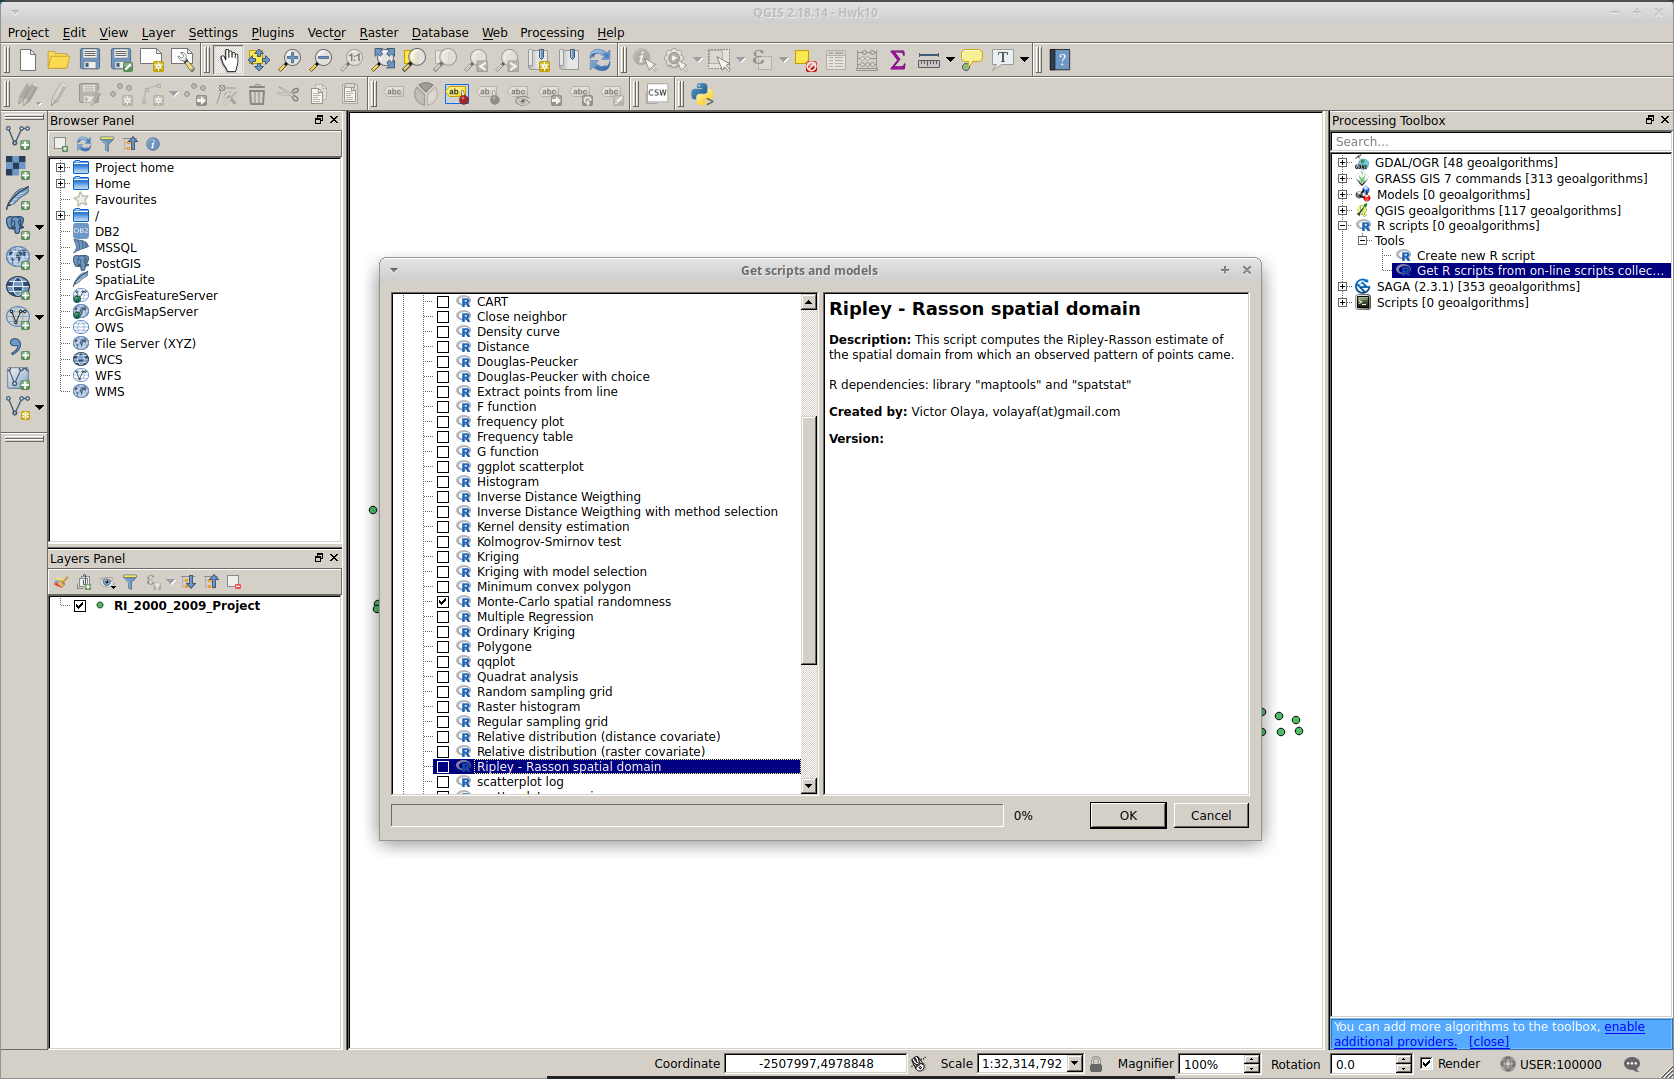
\includegraphics{images/installRscripts.png}
\caption{Installing R-scripts in QGIS}
\end{figure}

and gave it a go:

\begin{figure}
\centering
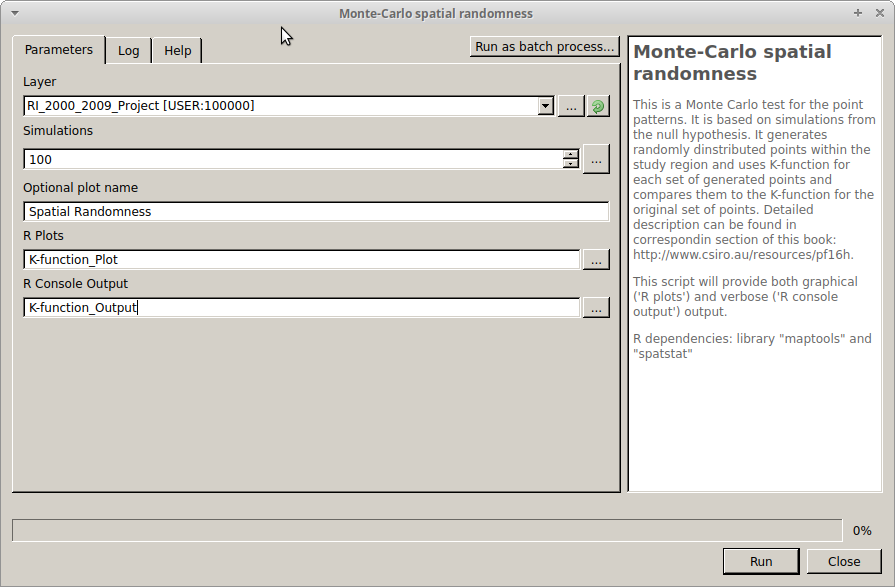
\includegraphics{images/Monte-Carlo.png}
\caption{K-function in QGIS}
\end{figure}

I watched as 100 trials ran, but I the output came back empty. My hunch
is that I am missing R-libraries that render graphics and tables. Given
enough time, I am confident I could get this to work using QGIS.

Since I have a final project that I need to focus on, however, I'm going
to leave this where it is.

\vskip 0.2in


    \begin{quote}
\begin{enumerate}
\def\labelenumi{(\arabic{enumi})}
\setcounter{enumi}{1}
\tightlist
\item
  A plot of both expected and observed K values with envelope curves by
  using 99 permutation. (5 points)
\end{enumerate}
\end{quote}

\vskip 0.2in


    \begin{quote}
\begin{enumerate}
\def\labelenumi{(\arabic{enumi})}
\setcounter{enumi}{2}
\tightlist
\item
  Discuss the results on the spatial pattern and its relation to the
  distance. (5 points)
\end{enumerate}
\end{quote}

\vskip 0.2in


    \begin{quote}
(Optional/open end/extra credit) Tune the parameters and options in the
ArcGIS for the K-function and discuss the resulting differences
(quantitative/qualitative) due to the change of parameters and
selection. (1-x points)
\end{quote}

\vskip 0.2in


    \hypertarget{notes-on-the-science-part}{%
\subsubsection{Notes on the science
part:}\label{notes-on-the-science-part}}

SHIPS (Statistical Hurricane Intensity Prediction Scheme) model for TC
intensity forecasting is derived by regression analysis from a set of
selected parameters sets (DeMaria \& Kaplan 1994, 1999; DeMaria et
al.~2005). The SHIPS data files can be found at
ftp://rammftp.cira.colostate.edu/demaria/SHIPS/. One of the data files
for the period 1989-2009 hurricane season can be downloaded at
ftp://rammftp.cira.colostate.edu/demaria/SHIPS/2010/lsdiaga\_1982\_2009\_rean\_biascorr\_sat.dat,
and the corresponding document file for this data file is also available
at
ftp://rammftp.cira.colostate.edu/demaria/SHIPS/2009/SHIPS\_predictor\_file\_2009.doc.
The original data are in ASCII but the data are hard to handle. Rapid
intensification (RI) is defined as rapid intensity increase in a short
time, typically 30 knots of wind increase in 24 hours (Kaplan and
DeMaria 2003; Yang et al.~2007; Kaplan et al.~2010). RI is relatively
rare cases with a probability around 5\% overall.

\hypertarget{references}{%
\subsubsection{References:}\label{references}}

Kaplan, J. and M. DeMaria (2003), Large-scale characteristics of rapidly
intensifying tropical cyclones in the North Atlantic basin, Wea.
Forecasting, 18, 1093-1108.

Kaplan, J., M. DeMaria, and J.A. Knaff (2010): A revised tropical
cyclone rapid intensification index for the Atlantic and east Pacific
basins. Wea. Forecasting, 25, 220-241.

Yang, R., J. Tang, and M. Kafatos (2007), ``Improved associated
conditions in rapid intensifications of tropical cyclones,'' Geophys.
Res. Lett., 34, L20807, doi:10.1029/2007GL031241.

DeMaria, M., and J. Kaplan, 1994b: A statistical hurricane intensity
prediction scheme (SHIPS) for the Atlantic basin, Wea. Forecasting, 9,
209-220.

DeMaria, M. and J. Kaplan, 1999: An Updated Statistical Hurricane
Intensity Prediction Scheme (SHIPS) for the Atlantic and Eastern North
Pacific Basins Mark, Wea. Forecasting, 14, 326--337.

DeMaria, M., M. Mainelli, L. K. Shay, J. A. Knaff, and J. Kaplan, 2005:
Further Improvements to the Statistical Hurricane Intensity Prediction
Scheme (SHIPS), Wea. Forecasting, 20, 531--543.

\vskip 0.2in


    % Add a bibliography block to the postdoc
    
    
    
    \end{document}
